% Draft section for paper 1: the 52-week test (pre-registered 13 November 2026, docs/PAPER1_REVISION_PLAN.md).
% Not part of the arXiv or IJPE build until Karthik agrees. Build: cd paper/drafts && xelatex long_horizon.tex
% Numbers come from generated/lh_values.tex and generated/lh_tab.tex, written by
% scripts/make_long_horizon_tables.py from results/long_horizon/.
\documentclass[10pt,twocolumn,letterpaper]{article}
\usepackage[letterpaper,margin=0.72in,columnsep=0.28in]{geometry}
\usepackage{fontspec}
\setmainfont{TeX Gyre Pagella}
\usepackage{amsmath,booktabs,array,graphicx,adjustbox}
\usepackage[font=small,labelfont=bf,skip=6pt]{caption}
\usepackage{xcolor,colortbl}
\usepackage[verbose=silent]{microtype}
\usepackage{titlesec}
\definecolor{accent}{RGB}{38,78,120}
\definecolor{headtint}{RGB}{24,42,64}
\definecolor{wmcell}{RGB}{207,224,240}
\definecolor{lgbcell}{RGB}{250,222,196}
\definecolor{avgcell}{RGB}{214,234,214}
\newcommand{\secsquare}{\textcolor{accent}{\rule[0.14em]{0.52em}{0.52em}}\hspace{0.42em}}
\titleformat{\section}{\normalfont\large\bfseries\color{headtint}}{\secsquare\thesection}{0.45em}{}
\titleformat{\paragraph}[runin]{\normalfont\bfseries\color{headtint}}{}{0pt}{}[.]
\titlespacing*{\paragraph}{0pt}{6pt plus 2pt}{0.6em}
\newcommand{\lhSets}{seven}
\newcommand{\lhWmBest}{none}
\newcommand{\lhLgbBest}{five}
\newcommand{\lhAvgBest}{two}
\newcommand{\lhWmBeatsLgbBest}{none}
\newcommand{\lhLgbBestBeatsWm}{seven}
\newcommand{\lhPWmBetter}{1}
\newcommand{\lhPWmWorse}{24}
\newcommand{\lhPN}{48}
\newcommand{\lhPAvgWmBetter}{37}
\newcommand{\lhPAvgWmWorse}{0}
\newcommand{\lhPAvgLgbBetter}{8}
\newcommand{\lhPAvgLgbWorse}{9}
\newcommand{\lhGrowWmLo}{-0.065}
\newcommand{\lhGrowWmHi}{+0.237}
\newcommand{\lhFaWmLo}{95}
\newcommand{\lhFaWmHi}{118}
\newcommand{\lhGrowLgbLo}{-0.080}
\newcommand{\lhGrowLgbHi}{+0.150}
\newcommand{\lhFaLgbLo}{94}
\newcommand{\lhFaLgbHi}{112}
\newcommand{\lhGrowAvgLo}{-0.068}
\newcommand{\lhGrowAvgHi}{+0.134}
\newcommand{\lhFaAvgLo}{98}
\newcommand{\lhFaAvgHi}{111}

\begin{document}
\twocolumn[{\centering{\Large\bfseries\color{headtint} Forecasting 52 weeks ahead}\\[4pt]
{\small Draft section for paper 1, for review. Planned before it ran (13 November 2026).}\\[10pt]}]

\section{Forecasting 52 weeks ahead}

\textbf{Over 52 weeks the world model alone is not the most accurate forecast on any
data set. The average of the two models, each forecasting all 52 weeks at once, is
the most accurate on \lhLowestAvgDirect{} of \lhSets{} data sets, and LightGBM on the other three.}
Table~\ref{tab:long-horizon} and Figure~\ref{fig:long-horizon} give the scores. The test
was written down before it ran: the six Dominick's categories and M5, two windows of
52 weeks each (364 days on M5), the tuned settings of the final runs with only the
distance ahead changed, scored at every level as in the rest of the paper.

\paragraph{Main comparison, in blocks}
Each model forecasts 13 weeks, takes its forecast in as the sales of those weeks,
and forecasts the next 13, four times. Here the world model is clearly less
accurate than LightGBM in \lhPWmWorse{} of \lhPN{} paired comparisons and clearly more
accurate in \lhPWmBetter{}. Against the better of LightGBM's two setups on each data set it
is behind on \lhLgbBestBeatsWm{} of \lhSets{}. The average in blocks is clearly more accurate
than the world model alone in \lhPAvgWmBetter{} comparisons (clearly less in \lhPAvgWmWorse{}), and
than LightGBM in \lhPAvgLgbBetter{} (clearly less in \lhPAvgLgbWorse{}).

\paragraph{Taking in its own forecasts costs the world model most}
Forecasting all 52 weeks at once, the world model is more accurate than in blocks on
\lhDirectBeatsBlocksWm{} of \lhDirectSetsWm{} data sets; LightGBM is on \lhDirectBeatsBlocksLgb{} of \lhDirectSetsLgb{}. In blocks, the
world model's item by store error changes by \lhGrowWmLo{} to \lhGrowWmHi{} from the first 13
weeks to the last, LightGBM's by \lhGrowLgbLo{} to \lhGrowLgbHi{}. The world model rolls its state
forward from the sales it takes in; when those are its own forecasts, its errors are
carried into the state and grow with each block.

\paragraph{The rule carries to 52 weeks}
The paper's rule, the average of the two models, holds at 52 weeks when each model
forecasts the whole year at once. In paired tests the average forecasting directly is
clearly more accurate than LightGBM forecasting directly in \lhPAvgDirBetter{} of
\lhPAvgDirN{} comparisons and clearly less in \lhPAvgDirWorse{}; against the world model forecasting
directly it is clearly more accurate in \lhPAvgDirWmBetter{} and clearly less in \lhPAvgDirWmWorse{}.
These two comparisons were added after the planned ones.

\paragraph{Limits}
Two windows per data set and two retailers (six Dominick's categories and M5). The
plan is the one recorded, as everywhere in the paper. The settings were tuned for 8
weeks (28 days on M5) and not tuned again for 52. M5's world model was not run
forecasting all 52 weeks at once, because rolling its state 364 days in training is
beyond the compute of this test.

\begin{table*}[t]
\centering\footnotesize\setlength{\tabcolsep}{3pt}
\caption{Forecasts 52 weeks ahead (364 days on M5). WRMSSE over the 52 weeks, mean over levels and two windows, for
the world model (WM), LightGBM (LGB) and their average (Avg). In blocks: each model forecasts four blocks of 13 weeks,
each block's forecast taken in as sales before the next. Direct: each model forecasts all 52 weeks at once (not run for
M5's world model). Paired item bootstrap over levels and windows: comparisons clearly lower / clearly higher, of all.
Last four columns: WRMSSE item by store in the first and last block of 13 weeks, in blocks. Shading marks the lowest
of the six: \colorbox{wmcell}{world model}, \colorbox{lgbcell}{LightGBM}, \colorbox{avgcell}{average}.}
\label{tab:long-horizon}
\begin{adjustbox}{max width=\textwidth}\begin{tabular}{l ccc ccc cc cc cc}
\toprule
 & \multicolumn{3}{c}{In blocks} & \multicolumn{3}{c}{Direct} & \multicolumn{2}{c}{Paired} & \multicolumn{2}{c}{WM, item by store} & \multicolumn{2}{c}{LGB, item by store}\\
\cmidrule(lr){2-4}\cmidrule(lr){5-7}\cmidrule(lr){8-9}\cmidrule(lr){10-11}\cmidrule(lr){12-13}
Data set & WM & LGB & Avg & WM & LGB & Avg & WM vs LGB, blocks & Avg vs LGB, direct & Weeks 1 to 13 & 40 to 52 & Weeks 1 to 13 & 40 to 52\\
\midrule
Analgesics & 1.062 & \cellcolor{lgbcell}\textbf{0.865} & 0.907 & 0.964 & 0.867 & 0.868 & 0 / 3 of 8 & 1 / 0 of 8 & 0.697 & 0.686 & 0.696 & 0.683 \\
Bottled juice & 0.903 & 0.797 & 0.817 & 0.764 & 0.769 & \cellcolor{avgcell}\textbf{0.726} & 0 / 2 of 8 & 4 / 0 of 8 & 0.738 & 0.742 & 0.705 & 0.689 \\
Cheese & 1.086 & 0.689 & 0.820 & 0.773 & 0.707 & \cellcolor{avgcell}\textbf{0.677} & 0 / 8 of 8 & 2 / 0 of 8 & 0.701 & 0.938 & 0.692 & 0.738 \\
Frozen entrees & 0.424 & 0.397 & 0.393 & 0.412 & 0.393 & \cellcolor{avgcell}\textbf{0.387} & 0 / 5 of 8 & 2 / 0 of 8 & 0.469 & 0.404 & 0.450 & 0.370 \\
Soft drinks & 0.872 & 0.862 & 0.819 & 0.851 & \cellcolor{lgbcell}\textbf{0.754} & 0.767 & 1 / 0 of 8 & 0 / 2 of 8 & 0.618 & 0.767 & 0.631 & 0.781 \\
Snacks & 1.013 & 0.877 & 0.920 & 0.866 & 0.882 & \cellcolor{avgcell}\textbf{0.843} & 0 / 6 of 8 & 6 / 0 of 8 & 0.691 & 0.890 & 0.622 & 0.683 \\
M5 & 1.016 & 0.931 & 0.874 & n/a & \cellcolor{lgbcell}\textbf{0.839} & n/a & 4 / 14 of 24 & n/a & 0.823 & 1.000 & 0.849 & 0.908 \\
\bottomrule
\end{tabular}\end{adjustbox}
\end{table*}


\begin{figure*}[t]
\centering
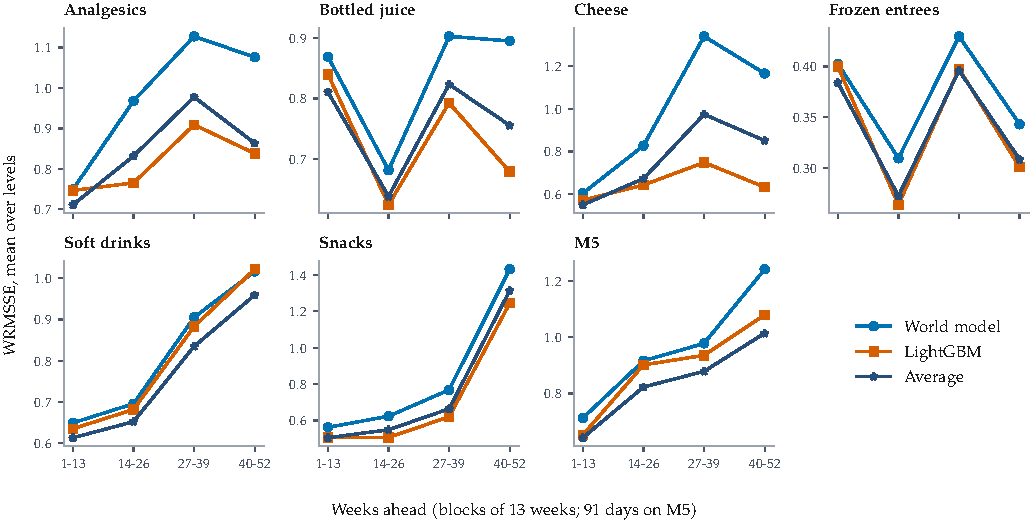
\includegraphics[width=\textwidth]{fig_long_horizon.pdf}
\caption{WRMSSE, mean over levels and two windows, in each block of 13 weeks (91 days
on M5), for the world model, LightGBM and their average forecasting in blocks.}
\label{fig:long-horizon}
\end{figure*}

\end{document}
